\documentclass[9pt]{beamer}

\usetheme{Warsaw}
%\usetheme{Szeged}
\usecolortheme{default}
\usefonttheme{structurebold}
\useinnertheme{rounded}

\usepackage[spanish]{babel}
\usepackage{amsmath}
\usepackage{amsfonts}
\usepackage{amssymb}

\usepackage{graphicx}

% \usepackage{tikz} % para poder realizar los graficos
\usepackage{verbatim}
% \usetikzlibrary{arrows,shapes} %para las flechas y nodos

\setbeamercovered{transparent}

\title{Desarrollo de un robot para la recolecci\'on de residuos}
%\subtitle{}
\institute[ITBA]{JAR 2010\\Ciudad de Buenos Aires\\ITBA\\

}

\date{3 de Noviembre de 2010}

\begin{document}

\frame{
	\titlepage
}

%================================== Outline ================================

\frame{
	\frametitle{Temario}

	\tableofcontents[part=1]
}

\part{Aspectos del desarrollo de un robot para la recolecci\'on de residuos}

\section{Introducci\'on}

	\subsection{¿Por qu\'e un robot recolector de residuos?}

		\frame{
			\frametitle{Principales motivaciones y objetivos}

			\begin{block} {¿Por qu\'e?}
				\begin{itemize}
					\item La recolecci\'on de basura es un problema log\'istico de grandes ciudades
					\item La acomulacion de basura alimenta animales transmisores de enfermedades
					\item Porque implica un desaf\'io tanto f\'isico como l\'ogico
					\item Porque servir\'ia como base y punto de partida a nuevos proyectos
				\end{itemize}
			\end{block}

			\begin{block} {Objetivos}
				Construir un robot m\'ovil capaz de identificar y recolectar residuos en un ambiente din\'amico
				como la terraza de la facultad.
				Desarrollar el soporte f\'isico, protocolo de comunicaci\'on, estructura de comportamientos
				y sistema de visi\'on.
			\end{block}

		}

\section{Arquitectura de procesamiento y comunicaciones}

	\subsection{Soporte f\'isico}

		\frame{
			\frametitle{Placas controladoras}
	
			\begin{block} {Placa controladora de motores DC}
				Permiten establecer la velocidad y sentido de giro del motor, registrar
				la informaci\'on del encoder del motor y conocer su consumo.
			\end{block}
	
			\begin{block} {Placa controladora de sensores}
				Obtener informaci\'on del entorno mediante distintos tipos de sensores.
				Utilizamos 8 tel\'emetros GP2D120, 3 sensores de proximidad CNY70 y 1
				sensor de distancia ultras\'onico SRF05. Tambi\'en tomamos lecturas de
				la carga de la bater\'ia.
			\end{block}
	
			\begin{block} {Placa controladora de servos}
				Dise\~nada pero no implementada. Controla hasta 5 servo motores digitales.
			\end{block}
	
		}

		\frame{
			\frametitle{Diagrama interior, placas controladoras de motores y sensores}
	
			\begin{figure}
				\centering
				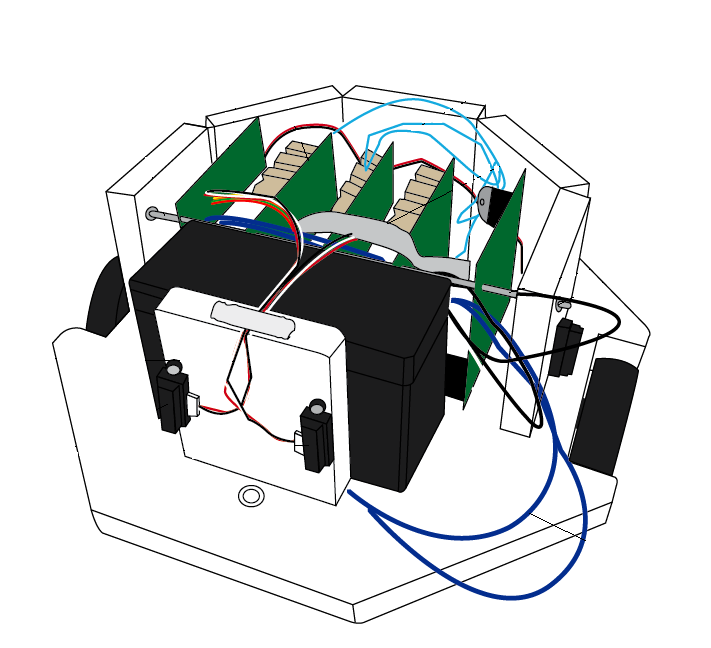
\includegraphics[scale=.20]{desarme_i.png}
				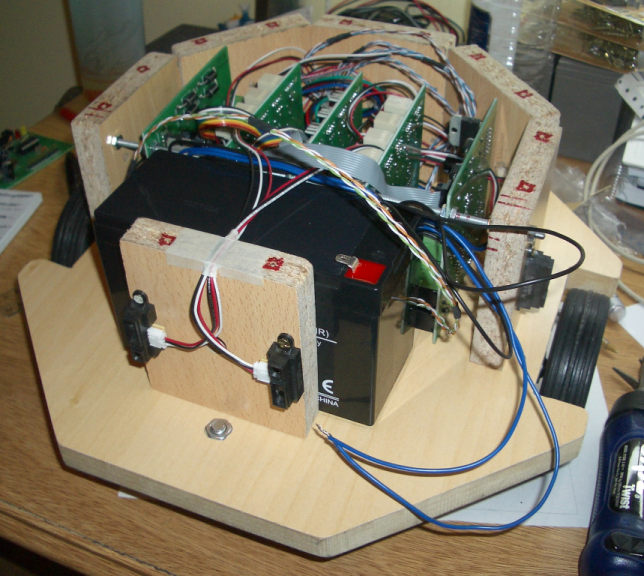
\includegraphics[scale=.20]{placas.png}
			\end{figure}
		}

	\subsection{Protocolo de comunicaci\'on}

		\frame{
			\frametitle{Protocolo de comunicaci\'on}
	
			\begin{block} {Protocolo de comunicaci\'on}
				El protocolo permite la comunicaci\'on entre el controlador principal y las
				placas que controlan los motores y obtienen datos del entorno.

				Mediante una configuraci\'on de Daisy-Chain entre las placas, transporta los
				comandos y respuestas.
			\end{block}

			\begin{figure}
				\centering
				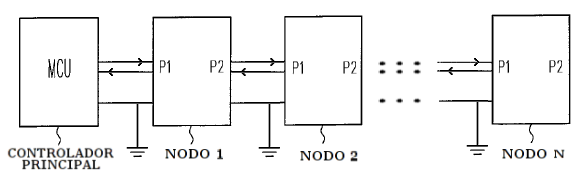
\includegraphics[scale=.2]{daisychain_diagram.png}
			\end{figure}

			\begin{block} {Elementos del paquete}
				Formato y encabezado del paquete de datos	

				\begin{table}[h]
					\begin{center}
						\begin{tabular}{|c|c|c|c|c|c|}
							\hline
							LARGO & DESTINO & ORIGEN & COMANDO & DATO & XOR\\
							\hline
						\end{tabular}
					\end{center}
				\end{table}

			\end{block}

		}

\section{Arquitectura de comportamientos}

	\subsection{¿C\'omo est\'a compuesta?}

		\frame{
			\frametitle{Arquitectura de comportamientos}
	
			\begin{block} {Elementos principales}
				La arquitectura de comportamientos elegida fue subsumption desarrollada por Rodney Brooks.
				B\'asicamente distintos est\'imulos activan o no ciertos comportamientos con prioridades
				diferentes.
			\end{block}
	
			\begin{figure}
				\centering
				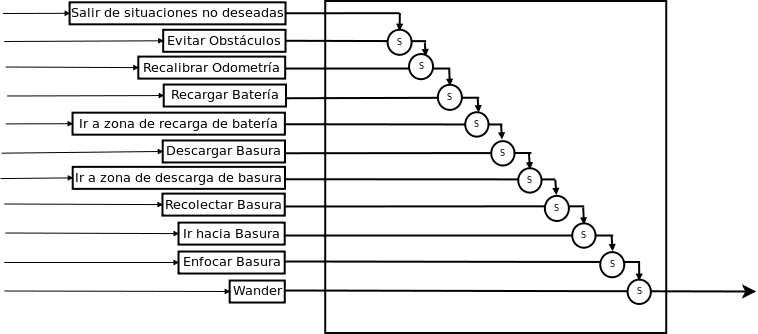
\includegraphics[scale=.3]{behavioursArchitecture2.png}
			\end{figure}

		}

		\frame{
			\frametitle{Estructura de los comportamientos: Subsumption}
	
			\begin{block} {Arquitectura de comportamientos}
				\begin{itemize}
					\item \textbf{Salir de situaciones no deseadas}: Evita el atascamiento.
					\item \textbf{Evitar obst\'aculos}: Acciona los motores seg\'un informaci\'on de los sensores.
					\item \textbf{Recalibrar odometr\'ia}: Utiliza landmarks para calibrar su posici\'on.
					\item \textbf{Recargar bater\'ia}: Mecanismo para recargarse en la base.
					\item \textbf{Ir a zona de recarga}: Navega hacia la l\'inea mas cercana y luego realiza line-following para llegar a la zona de recarga.
					\item \textbf{Descargar basura}: Mecanismo de descarga.
					\item \textbf{Ir a zona de descarga}: Navega hacia la l\'inea mas cercana y luego realiza line-following para llegar a la zona de recarga.
					\item \textbf{Recolectar basura}: Activa el mecanismo de recolecci\'on.
					\item \textbf{Ir hacia basura}: Desplaza al robot hacia las cercan\'ias de un residuo.
					\item \textbf{Enfocar basura}: Desplaza al robot hasta que la basura se encuentre centrada.
					\item \textbf{Wander}: Recorre el entorno  en búsqueda de residuos.
				\end{itemize}
			\end{block}
		}

	\subsection{Simulaci\'on}

		\frame{
			\frametitle{Simulaci\'on del ambiente}

			\begin{block} {Herramienta}
				Para la simulaci\'on del ambiente utilizamos Webots.
			\end{block}
	
			\begin{figure}
				\centering
				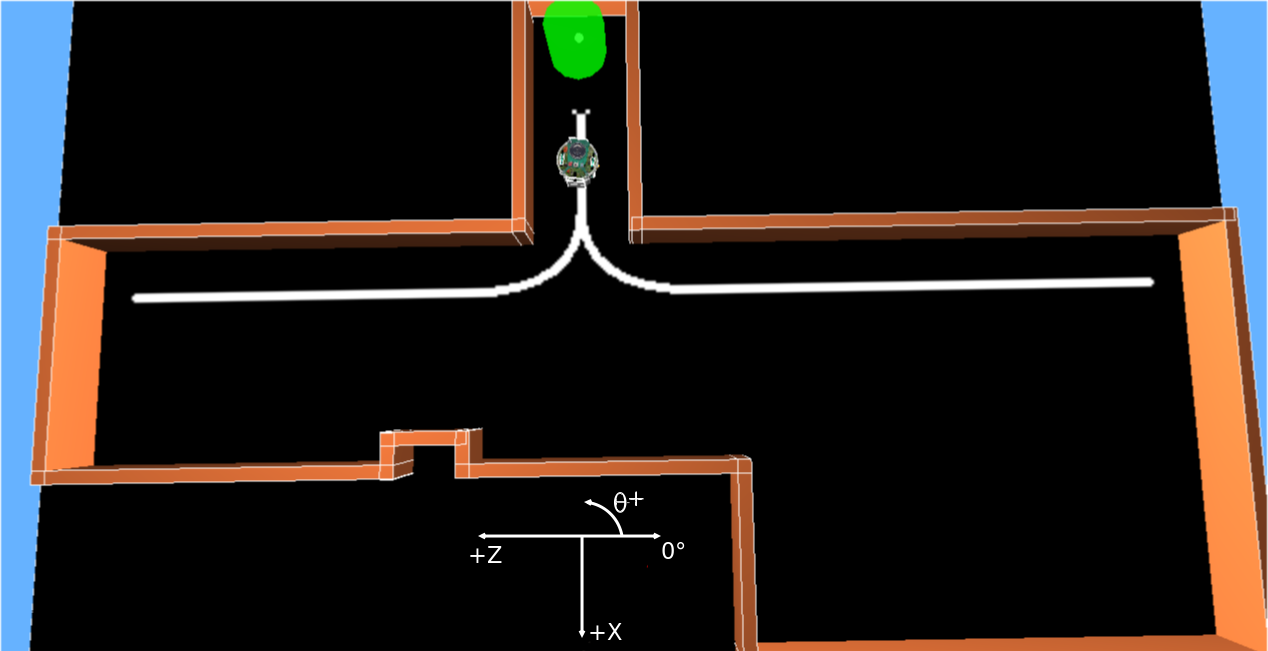
\includegraphics[scale=.15]{arenafinal.png}
				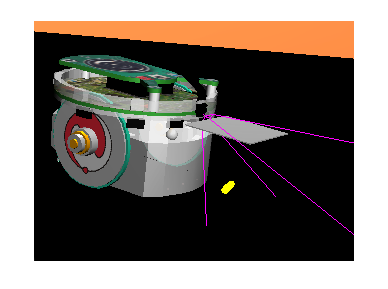
\includegraphics[scale=.3]{collect4.png}
			\end{figure}
		}

\section{Sistema de visi\'on}

	\subsection{¿C\'omo est\'a compuesto?}

		\frame{
			\frametitle{Sistema de visi\'on}
		
			\begin{block} {Elementos principales}
				Las im\'agenes captadas por la c\'amara son procesadas por una serie de algor\'itmos en C++ y la librer\'ia
				de visi\'on computacional OpenCV.
			\end{block}

			\begin{block} {Sistema de filtros}
				\begin{itemize}
					\item \textbf{Filtro de color}: Elimina pixeles que no posean un color dentro del rango de inter\'es.
					\item \textbf{Dilataci\'on-erosi\'on}: Eliminaci\'on de ruido, realce de caracter\'isticas.
					\item \textbf{Umbral}: Elimina componentes d\'ebiles.
					\item \textbf{Identificador de contornos}: Extracci\'on y representaci\'on de bordes con pol\'igonos.
					\item \textbf{Filtros de contorno}: Analiza distintos par\'ametros (\'area, per\'imetro, excentricidad)
					para determinar si es un objeto de inter\'es.
				\end{itemize}
			\end{block}
		}

		\frame{
			\frametitle{Estructura del algor\'itmo de visi\'on y figura explicativa}
	
			\begin{figure}
				\centering
				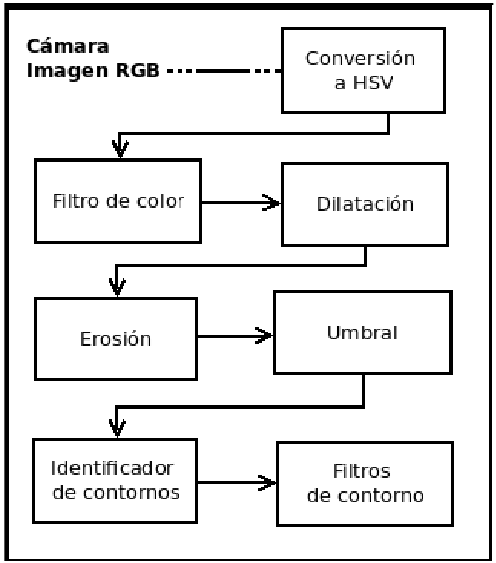
\includegraphics[scale=.25]{algoVision.png}
				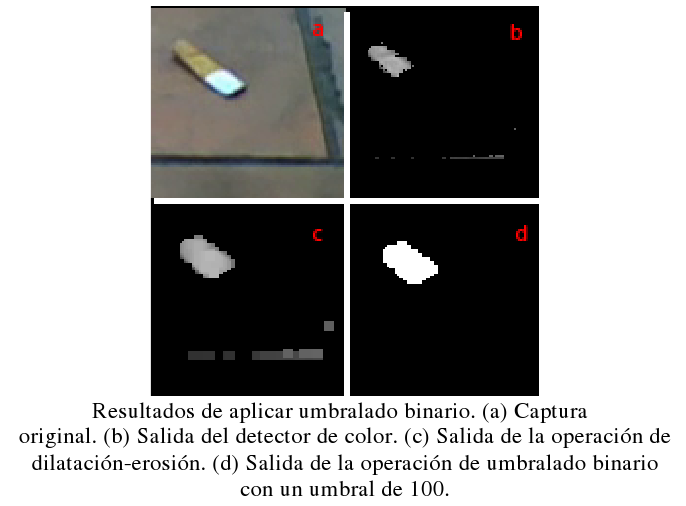
\includegraphics[scale=.25]{picVision.png}
			\end{figure}
		}
\section{Conclusiones}

	\frame{
		\frametitle{Conclusiones}

		\begin{block} {Conclusiones}
			El testeo tanto del hardware como del software hasta ahora implementados son alentadores.
			Queda mucho trabajo por realizar pero creemos que la mayor contribuci\'on se encuentra en
			el proyecto de incorporaci\'on progresiva de tecnolog\'ia para el dise\~no, construcci\'on,
			experimentaci\'on e investigaci\'on en rob\'otica e inteligencia computacional en del CENCOM
			del Departamento de Ingenier\'ia Inform\'atica del ITBA.
		\end{block}

		\begin{block} {SVN del proyecto}
			P\'agina del proyecto: http://code.google.com/p/tpf-robotica/
		\end{block}

	}

\end{document}